% !TEX TS-program = pdflatex
% !TEX root = tesi.tex

\documentclass[
  a4paper,
  twoside,
  openright,
  titlepage,
  headinclude,
  footinclude,
  BCOR5mm,
  numbers=noenddot,
  cleardoublepage=empty,
  tablecaptionabove
]{scrreprt}

\usepackage[T1]{fontenc}
\usepackage[utf8]{inputenc}
\usepackage[english,italian]{babel}
\usepackage{amsmath,amssymb}
\usepackage{indentfirst}
\usepackage[
  style=philosophy-modern,
  hyperref
]{biblatex}
\usepackage{chngpage}
\usepackage{calc}
\usepackage{listings}
\usepackage{graphicx}
\usepackage{subfig}
\usepackage{lipsum}
\usepackage{shapepar}
\usepackage{pifont}
\usepackage[
  eulerchapternumbers,
  subfig,
  beramono,
  eulermath,
  pdfspacing,
  listings
]{classicthesis}
\usepackage{arsclassica}
\usepackage{tikz}

% FONT UTILIZZATO DAL CONSERVATORIO
\usepackage[defaultfam,tabular,lining]{montserrat} %% Option 'defaultfam'
%% only if the base font of the document is to be sans serif
\usepackage[T1]{fontenc}
\renewcommand*\oldstylenums[1]{{\fontfamily{Montserrat-TOsF}\selectfont #1}}

\usepackage{ccicons}

% ********************************************************************
% Personal commands
% ********************************************************************
\DeclareRobustCommand*{\clsname}[1]{{\normalfont\sffamily#1}}
\DeclareRobustCommand*{\pkgname}[1]{{\normalfont\sffamily#1}}
\DeclareRobustCommand*{\optname}[1]{{\normalfont\ttfamily#1}}
\DeclareRobustCommand*{\cmdname}[1]{\mbox{\lstinline[basicstyle=\normalsize\ttfamily]!\\#1!}}

\DeclareRobustCommand*{\classicthesis}{Classic\-Thesis}
\DeclareRobustCommand*{\arsclassica}{{\normalfont\sffamily ArsClassica}}

% ********************************************************************
% Hyper-references
% ********************************************************************
\newcommand{\mail}[1]{\href{mailto:#1}{\texttt{#1}}}


% ********************************************************************
% Graphics
% ********************************************************************
\graphicspath{{Graphics/}}


% ********************************************************************
% Code
% ********************************************************************
\definecolor{lightergray}{gray}{0.99}
\definecolor{bbari}{cmyk}{1,0.44,0,0.28}

\lstset{language=[LaTeX]Tex,
     keywordstyle=\color{RoyalBlue},
     basicstyle=\small\ttfamily,
     commentstyle=\color{Emerald}\ttfamily,
     stringstyle=\rmfamily,
     numberstyle=\scriptsize,
     showstringspaces=false,
     breaklines=true,
     frame=lines,
     backgroundcolor=\color{lightergray},
     flexiblecolumns=true,
     escapeinside={�*}{*�},
     firstnumber=last,
}

\newcommand{\meta}[1]{$\langle${\normalfont\itshape#1}$\rangle$}

\lstset{	morekeywords=%
    {ProvidesPackage,RequirePackage,areaset,ifthenelse,%
     chapterNumber,undefined,boolean,DeclareRobustCommand,%
     spacedallcaps,textssc,MakeTextUppercase,lehead,%
     microtypesetup,textls,spacedlowsmallcaps,MakeTextLowercase,%
     sodef,allcapsspacing,lowsmallcapsspacing,thesection,%
     color,headmark,rohead,headfont,pnumfont,titleformat,%
     part,partname,thepart,chapter,thechapter,titlerule,%
     subsection,thesubsection,subsubsection,thesubsubsection,%
     paragraph,theparagraph,descriptionlabel,titlespacing,%
     formatchapter,textcolor,clearscrplain,rofoot,labelitemi,
     captionsetup,hypersetup}}

\lstnewenvironment{code}%
   {\setkeys{lst}{columns=fullflexible,keepspaces=true}%
   \lstset{basicstyle=\small\ttfamily}}{}


% ********************************************************************
% Bibliography
% ********************************************************************
\bibliography{Bibliography}

\defbibheading{bibliography}{%
\cleardoublepage
\manualmark
\phantomsection
\addcontentsline{toc}{chapter}{\tocEntry{\bibname}}
\chapter*{\bibname\markboth{\spacedlowsmallcaps{\bibname}}
{\spacedlowsmallcaps{\bibname}}}}

\renewcommand*{\nameyeardelim}{\addcomma\space}


\newcommand{\myName}{Francesco Vittorio Maria Dicorato}
\newcommand{\myTitle}{Ambisonics Videoludico 3D}
\newcommand{\mySubTitle}{IMPLEMENTAZIONE IN AMBIENTE UNITY}

\begin{document}
\pagenumbering{roman}
\pagestyle{plain}
% !TEX TS-program = pdflatex
% !TEX root = ../tesi.tex

%*******************************************************
% Titlepage
%*******************************************************
\begin{titlepage}
\pdfbookmark{Titlepage}{Titlepage}
\changetext{}{}{}{((\paperwidth  - \textwidth) / 2) - \oddsidemargin - \hoffset - 1in}{}
  \begin{center}
    {\LARGE
      
\includegraphics[width=0.641\textwidth]{logo.eps} \\[0.5cm]

      {\normalsize{DIPARTIMENTO DI NUOVE TECNOLOGIE E LINGUAGGI MUSICALI}} \\[-0.2cm]
      {\spacedlowsmallcaps{Scuola di Musica elettronica}} \\[0.5cm]

      {\normalsize{DIPLOMA ACCADEMICO DI PRIMO LIVELLO IN}} \\[-0.2cm]
      {\spacedlowsmallcaps{Musica Elettronica}} \\[1.414cm]
      %{\spacedlowsmallcaps{Musica Elettronica}} \\[2cm]

      {\huge{\spacedlowsmallcaps{\myName}}}\vspace{-0.3cm}
      \par\noindent\rule{\textwidth}{0.4pt}\vspace{0.3cm}
      {\Huge{\color{bbari}\spacedallcaps{\myTitle}}}
      \par\noindent\rule{\textwidth}{0.4pt}\vspace{0.3cm}
      {\spacedlowsmallcaps{\mySubTitle}}
    }

    \vspace{2.718cm}

    \begin{minipage}[t]{0.49\textwidth}
    \begin{flushleft} \large
    \emph{Autore:}\\
    \spacedlowsmallcaps{\myName}\\
    \spacedlowsmallcaps{755/T}
    \end{flushleft}
    \end{minipage}
    \begin{minipage}[t]{0.49\textwidth}
    \begin{flushright} \large
    \emph{Relatore:} \\
    \spacedlowsmallcaps{Prof. Giuseppe Silvi}\\
    \spacedlowsmallcaps{Elettroacustica}
    \end{flushright}
    \end{minipage}\\[0.5cm]
    \begin{minipage}[t]{0.99\textwidth}
    \begin{flushright} \large
    \emph{Correlatore:} \\
    \spacedlowsmallcaps{Luigi Nono}\\
    \spacedlowsmallcaps{Compositore}
    \end{flushright}
    \end{minipage}\\[3cm]

    \vfill

    ANNO ACCADEMICO 2022/23

  \end{center}
\end{titlepage}

% !TEX TS-program = pdflatex
% !TEX root = ../tesi.tex

%*******************************************************
% Titleback
%*******************************************************
\thispagestyle{empty}
\pdfbookmark{Titleback}{Titleback}

\hfill

\vspace{\stretch{2}}

\begin{center}
\myName \\
\smallskip
\textit{\myTitle}\\
\smallskip
Copyright \ccbyncsa\\
2022-2023
\end{center}
\vspace{\stretch{1}}

\medskip

%\noindent\textsf{\spacedlowsmallcaps{Disclaimer}} \\
%\noindent
%Questo lavoro è stato realizzato con \LaTeX{} su Windows usando \arsclassica, un rielaborato dello stile \classicthesis{} ideato da Andr\'e Miede, ispirato al capolavoro \emph{The Elements of Typographic Style} di Robert Bringhurst.
%
%\bigskip

%\noindent I nomi commerciali, i loghi e i marchi registrati menzionati nella guida appartengono ai rispettivi proprietari, i pacchetti e le relative documentazioni ai rispettivi
%autori.

\bigskip

\noindent
\textsf{\spacedlowsmallcaps{Contatti}}

\noindent
{\raisebox{-0.33ex}{\ding{43}}}\,\mail{francesco.dicorato@hotmail.it}

\cleardoublepage
% !TEX TS-program = pdflatex
% !TEX root = ../tesi.tex

%*******************************************************
% Acknowledgements
%*******************************************************
\pdfbookmark{Acknowledgements}{Acknowledgements}

\chapter*{Riconoscimenti}

\begin{flushright}
\itshape
I videogiochi sono uno strumento che ci permette di entrare in contatto con altri universi. \\
Grazie ai supporti tecnologici è quindi possibile sperimentare qualcosa che va ben oltre il mondo reale. \\
È come quando si legge un libro appassionante, \\
ma lo stesso effetto si può provare quando si ascolta della musica oppure si guarda un film. \\
Allo stesso modo, attraverso i videogiochi si può entrare in contatto con degli universi paralleli, \\
ma soprattutto si può vivere questa esperienza in modo più coinvolgente e personale.
I videogiochi hanno questa forza. \\


\medskip
--- Kazunori Yamauchi

\end{flushright}

\bigskip
\bigskip

\heartpar{Voglio ringraziare tutti coloro che hanno permesso che questo giorno arrivasse, in maniera diretta e indiretta, in particolar
modo la mia famiglia, che è costituita da familiari ed amici, i miei colleghi ed i Maestri che mi hanno aiutato a raggiungere questo splendido traguardo.
Ringrazio mia madre per la sua pazienza, la sua fiducia e gli sforzi che ha impiegato nel sostenermi, i quali si sono rivelati particolarmente
cruciali nell'ultima fase di questo percorso, la più importante. Ringrazio mio padre per il suo sostegno da tutti i punti di vista, il quale,
a suo modo, è definibile come una carica di nuovo vigore quando le motivazioni sembrano mancare.
Ringrazio i miei fratelli Enrico, Luigi e Domenico, i quali si sono dimostrati una fonte di supporto e di crescita anche a livello personale, psicologico e morale. Tra di loro,
voglio considerare anche Zio Mimmo che è sempre stato presente con la sua ironia, la sua disponibilità e le sue cariche mattutine!
Per me è un fratello o una sorella, anche chi non ha un legame di sangue, perchè di persone così belle è difficile trovarne qualcuna: X6, Comix, Bau!
Vi voglio bene: Alessandro C., Nicola, Vito D., Alberto, Rino Dil., Mela, Luigi, Vito M., Francesca, Giusy, Antonella, Dory, Nicole, Savino, Rosa, Pio, Angelo G., Angelo I., Claudia, Ale D, Rino Dib..
Sottolineo ed evidenzio i miei ringraziamenti per Mela, per il suo lavoro grafico, per il suo contributo e per il sostegno quotidiano che mi ha portato a terminare questo progetto.
Siete stati tutti quanti importanti nella mia vita, incisa da voi con un vostro marchio dal calco di maggiore o minore spessore, ma egualmente significante.}

\pagestyle{scrheadings}
% !TEX TS-program = pdflatex
% !TEX root = ../tesi.tex

%*******************************************************
% Contents
%*******************************************************
\phantomsection
\pdfbookmark{\contentsname}{tableofcontents}
\setcounter{tocdepth}{2}
\tableofcontents
\markboth{\spacedlowsmallcaps{\contentsname}}{\spacedlowsmallcaps{\contentsname}}

\cleardoublepage
\pagenumbering{arabic}
% !TEX TS-program = pdflatex
% !TEX root = ../tesi.tex

%************************************************
\chapter{ABSTRACT}
\label{chp:abstract}
%************************************************

Questo progetto prevede l'utilizzo della metodologia Ambisonics per il mixing e la produzione tridimensionale dell'audio all'interno di un percorso videoludico 3D, riprodotto mediante l'uso del motore grafico Unity per lo sviluppo del contenuto interattivo e di animazione visiva. \\
Ambisonics di ordine superiore ha trovato un mercato di nicchia nei videogiochi sviluppati da Codemasters. \\
 Il loro primo gioco a utilizzare un motore audio Ambisonic è stato "Colin McRae: DiRT”
Le prime musiche per videogiochi erano generalmente monofoniche, suonate adoperando apparecchiature quali computer e sintetizzatori, e venivano messe in loop, oppure riprodotte fra un livello e l'altro. \\
Alcuni esempi includono i titoli di Pac-Man della Namco (1980) composti da Toshio Kai. \\
 Il primo videogioco a presentare una colonna sonora dotata di un sottofondo continuo fu quella di Space Invaders della Taito Corporation (1978), realizzata da Tomohiro Nishikado. A partire dal 1980, alcuni videogiochi iniziarono ad adoperare apparecchiature digitali, campionamenti e sintesi FM per fare musica. \\
Rally-X della Namco, uscito nel 1980,
fu probabilmente il primo videogame a presentare una colonna sonora realizzata con un convertitore di segnale analogico (DAC) per riprodurre note campionate. \\
Mentre le console casalinghe si avvicinavano alla quarta generazione (o era dei 16-bit),
il compositore Yuzo Koshiro utilizzò l'hardware del Mega Drive per comporre "brani progressivi, techno, e orecchiabili molto evoluti". \\
A partire dagli anni `90, la musica per videogiochi iniziò a presentare sonorità realizzate con strumenti musicali veri e propri. \\
La musica per videogiochi arrivò ad amalgamarsi, infine, coi mondi musicali del pop, hip ed electro. \\
La mia personale aggiunta storica, dal punto di vista musicale, avvalendomi del metodo Ambisonics, sarà quella di inserire una composizione del genere "Computer Music", come novità, all'interno di una rappresentazione videoludica. \\

% !TEX TS-program = pdflatex
% !TEX root = ../tesi.tex


%************************************************
\chapter{Ambisonics}
\label{chp:Ambisonics}
%************************************************

Ambisonics è un formato audio surround a sfera completa: oltre al piano orizzontale, copre le sorgenti sonore sopra e sotto l'ascoltatore.
\begin{itemize}
\item Il \textbf{surround} (dal verbo inglese "to surround", in italiano "circondare", o più propriamente "avvolgere") è l'informazione sonora che in una tecnica di riproduzione/registrazione del suono (ad esempio la quadrifonia) costituisce il fronte sonoro alle spalle dell'ascoltatore.\\ Il surround, in abbinamento al fronte sonoro anteriore, ha lo scopo di collocare l'ascoltatore al centro della scena sonora, offrendo quindi la possibilità di un maggior realismo sonoro, in quanto normalmente in natura il suono raggiunge l'ascoltatore da ogni direzione.\\
\end{itemize}

\begin{figure}[h]
      \centering
      
\includegraphics[width=0.3\textwidth]{Graphics/AmbisonicLogo.png}
      \caption{⟨Logo simbolico Ambisonics⟩}
      \label{fig:⟨etichetta⟩}
      \end{figure}

\section{Premessa storica}

Michael Gerzon fece dichiarazione senza compromessi nel suo articolo intitolato
\textit{\textbf{What’s wrong with quadraphonics?}} nel Maggio del 1974 sulla rivista Studio Sound.\\
L’attacco principale che portava a questi sistemi era l’apparente localizzazione dei
suoni affidata all’immaginazione dell’ascoltatore.\\
Dopo aver catalogato i continui difetti delle registrazioni quadrifoniche, ha
continuato descrivendo un nuovo approccio alla riproduzione del suono surround,
noto come sistemi di ”\textbf{sintesi armonica}” o ”\textbf{kernel}”.\\
 Il nuovo approccio è iniziatodall’osservazione che gli effetti che si vorrebbe produrre includono un continuum
di direzioni attorno all’ascoltatore. Tali sistemi immaginano un numero
limitato di canali utilizzati per trasmettere il suono all’ascoltatore, ma sono progettati
per ricreare una gamma continua di direzioni attorno all’ascoltatore che
si avvicinano all’originale. La matematica utilizzata non è algebra ”matriciale”
(che è usata solo per descrivere trasformazioni di un numero finito di variabili)
ma algebra ”kernel” (che è la matematica corrispondente usata quando si ha un
continuum infinito di variabili).\\
Ha spiegato di essere stato recentemente associato al sistema Ambisonic, che
era un esempio di sistema kernel.\\ È stato sostenuto dalla \textbf{National Research and
Development Corporation} (\textbf{NRDC}) e ha coinvolto il professor Peter Fellgett della
Reading University.\\
Il sistema audio surround britannico Ambisonics esiste da quasi trent’anni.\\
Nonostante la mancanza del finanziamento delle principali società disponibili
per i sistemi concorrenti, Ambisonics è sopravvissuta grazie a prestazioni tecniche
superiori e al supporto di appassionati di tutto il mondo.\\
Con la facile disponibilità di una potente elaborazione del segnale digitale
 (al contrario dei circuiti analogici costosi e soggetti a errori che dovevano essere utilizzati durante i suoi primi anni)
 e il successo dell'introduzione sul mercato dei sistemi audio surround home theater sin dagli anni '90,
  l'interesse per Ambisonics tra ingegneri del suono, sound designer, compositori, società di media,
  emittenti e ricercatori è tornato e continua ad aumentare.

  \section{Introduzione}
Ambisonics può essere inteso come un'estensione tridimensionale dello stereo M/S (mid/side),
aggiungendo ulteriori canali di differenza per altezza e profondità.\\
Il set di segnali risultante è chiamato \textbf{formato B}.
I suoi canali componenti sono etichettati \textbf{W} per la pressione sonora (la M in M/S),
\textbf{X} per il gradiente di pressione sonora anteriore-meno-posteriore, 
\textbf{Y} per sinistra- meno-destra (la S in M/S) e \text{Z} per su-meno-giù. \\
Il segnale \textbf{W} corrisponde a un microfono omnidirezionale,
mentre \textbf{XYZ} sono le componenti che sarebbero captate da
capsule a forma di otto orientate lungo i tre assi spaziali.

\section{Panning di una sorgente}
Un semplice panner Ambisonic (o codificatore) prende un segnale sorgente S e due parametri,
 l'angolo orizzontale $\theta$ e l'angolo di elevazione $\phi$.\\
 Posiziona la sorgente all'angolo desiderato distribuendo il segnale sui 
 componenti Ambisonic con guadagni diversi:

 \begin{equation}
W =S\cdot\frac{1}{\sqrt{2}}
 \end{equation}

 \begin{equation}
      X=S\cdot\cos\theta\cos\phi
\end{equation}

\begin{equation}
      Y =S\cdot\sin\theta\cos\phi
\end{equation}

\begin{equation}
      Z=S\cdot\sin\phi
\end{equation}
\\

Essendo omnidirezionale, il canale W riceve sempre lo stesso segnale di ingresso costante, indipendentemente dagli angoli. \\
Affinché abbia più o meno la stessa energia media degli altri canali, W è attenuato di circa 3 dB (appunto, diviso per la radice quadrata di due).\\
 I termini per XYZ in realtà producono gli schemi polari dei microfoni a forma di otto. \\ 
 Prendiamo il loro valore $\theta$ e $\phi$ e moltiplichiamo il risultato per il segnale di ingresso.\\
  Il risultato è che l'ingresso finisce in tutti i componenti esattamente come l'avrebbe captato il microfono corrispondente.

\subsection{Microfoni virtuali}

I componenti in formato B possono essere combinati per derivare microfoni virtuali con qualsiasi diagramma polare di primo ordine (omnidirezionale, cardioide, ipercardioide, figura di otto o qualsiasi altra via di mezzo) che punta in qualsiasi direzione.
 \\È possibile derivare contemporaneamente più microfoni di questo tipo con parametri diversi, per creare coppie stereo coincidenti (come un Blumlein) o array surround.

 \begin{center}
 \captionsetup{type=table}
 \captionof{table}{Un microfono virtuale orizzontale ad angolo orizzontale $\theta$ con Pattern $0\le p\le 1$ dato da
 $M(\theta,p)=p{\sqrt{2W}}+(1-p)(\cos\theta X+\sin\theta Y)$.
 Questo microfono virtuale è normalizzato in campo libero,
  il che significa che ha un guadagno costante di uno per i suoni in asse. }
\begin{tabular}{||p{3.0cm}|p{3.0cm}||} 
      \hline\hline
      p & Pattern \\
      \hline\hline
      0 & Figura a 8 \\
      \hline\hline
      (0, 0.5) & Iper e Super-cardioide\\
      \hline\hline
      0.5 & Cardioide \\
      \hline\hline
      (0.5, 1.0) & Cardioide Largo \\
      \hline\hline
      1.0 & Omnidirezionale \\
      \hline\hline
      \end{tabular}
\end{center}

I microfoni virtuali possono essere manipolati in post-produzione: i suoni desiderati possono essere individuati,
 quelli indesiderati soppressi e l'equilibrio tra suono diretto e riverberante può essere messo a punto durante il missaggio.
 
\section{Decoding di un segnale}

Un decoder Ambisonic di base è molto simile a un set di microfoni virtuali.
Per layout perfettamente regolari, è possibile generare un decodificatore semplificato puntando un microfono cardioide virtuale in direzione di ciascun altoparlante.
\\Ecco un quadrato:

\begin{equation}
      LF = ({\sqrt{2W}} + X + Y){\sqrt{8}}
\end{equation}

\begin{equation}
      LB = ({\sqrt{2W}} - X + Y){\sqrt{8}}
\end{equation}

\begin{equation}
      RB = ({\sqrt{2W}} - X - Y){\sqrt{8}}
\end{equation}

\begin{equation}
      RF = ({\sqrt{2W}} + X - Y){\sqrt{8}}
\end{equation}

\begin{figure}[h]
      \centering
      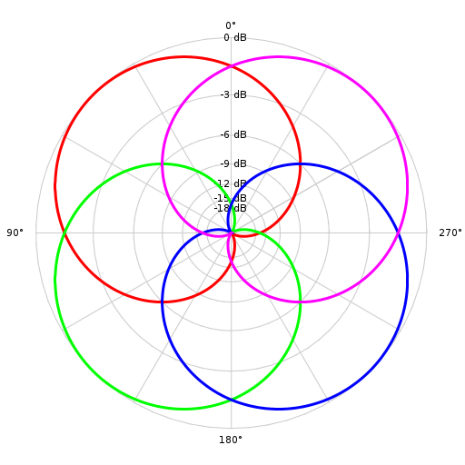
\includegraphics[width=0.8\textwidth]{Decodificatore.png}
      \caption{⟨Decodificatore basico in fase a banda singola per un layout di altoparlanti quadrati⟩}
      \label{fig:⟨etichetta⟩}
      \end{figure}

      In pratica, un vero decoder Ambisonic richiede una serie di ottimizzazioni psicoacustiche per funzionare correttamente.\\
      La decodifica dipendente dalla frequenza può anche essere utilizzata per produrre stereo binaurale;
      questo è particolarmente rilevante nelle applicazioni di realtà virtuale.
      
      \section{Gli ordini dell'Ambisonics}

      Nel contesto dei videogiochi, viene utilizzato principalmente l'ambisonics di primo ordine (o "B-format"), che consiste in quattro canali audio (W, X, Y e Z) che rappresentano rispettivamente il suono diffuso uniformemente nell'ambiente, e le tre dimensioni spaziali.\\
      Questo formato permette di ricostruire un campo sonoro 3D attraverso un numero variabile di altoparlanti, a seconda delle capacità e delle configurazioni dei sistemi di riproduzione sonora utilizzati.\\
      In genere, i videogiochi che supportano l'ambisonics di primo ordine consentono ai giocatori di selezionare il numero di altoparlanti utilizzati, in base alle loro esigenze e alle specifiche del sistema di riproduzione sonora che hanno a disposizione.\\
      Inoltre, gli sviluppatori di giochi possono utilizzare plugin o librerie di software dedicati per creare, manipolare e riprodurre il segnale ambisonico all'interno dell'ambiente di sviluppo del gioco.\\
      Il set di segnali risultante viene quindi chiamato Ambisonics di secondo, terzo o, collettivamente, di ordine superiore.\\
      Per un dato ordine $\mathbf{l}$, i sistemi a sfera completa richiedono componenti di segnale $(l+1)^{2}$ componenti, e $2l+1$ sono necessari per la riproduzione solo orizzontale.
\\
      \begin{figure}[h]
            \centering
            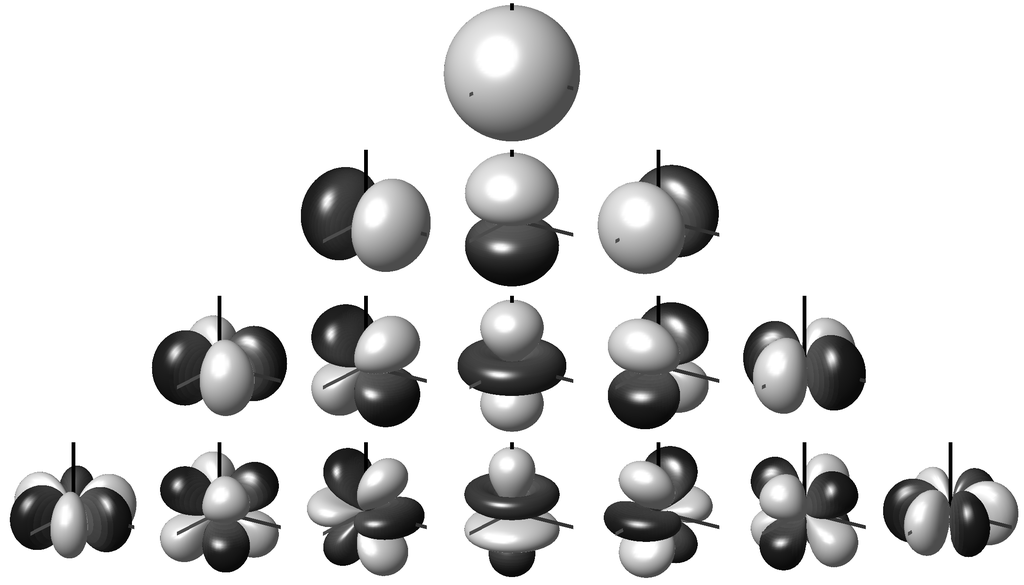
\includegraphics[width=0.8\textwidth]{OrdiniAmb.png}
            \caption{⟨Rappresentazione visiva dei componenti Ambisonic in formato B fino al terzo ordine.
            Le parti scure rappresentano le regioni in cui la polarità è invertita.
            Si noti come le prime due righe corrispondano ai modelli polari del microfono omnidirezionale e figura di otto.⟩}
            \label{fig:⟨etichetta⟩}
            \end{figure}

      \section{Problemi ed integrazioni}

      \subsection{Problemi}
      La risoluzione spaziale di Ambisonics di primo ordine come descritto sopra è piuttosto bassa.
      In pratica, ciò si traduce in sorgenti leggermente sfocate, ma anche in un'area di ascolto utilizzabile relativamente piccola o punto debole.\\
      La risoluzione può essere aumentata e lo sweet spot ampliato aggiungendo gruppi di componenti direzionali più selettivi al formato B.
      Questi non corrispondono più ai modelli polari convenzionali del microfono, ma sembrano piuttosto foglie di trifoglio. 
      
      L'utilizzo dell'Ambisonics nei videogiochi comporta alcune problematiche specifiche, tra cui:

      \begin{enumerate}
            \item Gestione del carico di lavoro del processore:
            L'elaborazione di un segnale audio in Ambisonics richiede una notevole quantità di potenza di elaborazione.
            In un videogioco, dove il processore deve gestire molte altre attività,
            questo può comportare una diminuzione delle prestazioni del gioco stesso
            
            \item Latenza: L'elaborazione in tempo reale di un segnale audio in Ambisonics può comportare un certo ritardo nella riproduzione del suono rispetto all'azione del gioco stesso.
            Questa latenza può influire sulla sensazione di immersività e può essere particolarmente problematica in giochi in cui la sincronizzazione audio-video è fondamentale.
            
\item Problemi di compatibilità: Non tutti i motori di gioco supportano l'Ambisonics, il che può limitare la sua applicazione in alcuni giochi.
Inoltre, la compatibilità con i diversi sistemi di riproduzione sonora può rappresentare una sfida per gli sviluppatori di giochi.

\item Gestione del volume: La riproduzione di un campo sonoro tridimensionale in Ambisonics comporta la gestione di più canali audio, il che può comportare difficoltà nella regolazione del volume di ogni singolo canale, soprattutto in situazioni in cui si desidera evidenziare un suono specifico o limitare il volume di altri suoni.
  
\item Codifica e decodifica: La codifica e decodifica di un segnale audio in Ambisonics richiede l'utilizzo di algoritmi specifici, che possono comportare una maggiore complessità nella produzione audio del gioco e un aumento del tempo e dei costi di sviluppo.

\end{enumerate}

\subsection{integrazioni}

Nonostante la limita disponibilità dei software e degli hardware disponibili per l'utilizzo di Ambisonics all'interno
dei videogiochi, esistono degli sviluppatori che hanno segnato una loro impronta storica in questo ambito sonoro:

\begin{enumerate}
      \item Unity: Unity è uno dei motori di gioco più popolari ed è ampiamente utilizzato per la produzione di giochi per molte piattaforme. Supporta l'Ambisonics attraverso plugin di terze parti come Facebook 360 Spatial Workstation e Steam Audio.
      \item Unreal Engine: Unreal Engine è un altro motore di gioco molto popolare, utilizzato per la produzione di molti giochi di successo. Supporta l'Ambisonics attraverso il plugin Steam Audio.
      \item FMOD Studio: FMOD Studio è un motore audio utilizzato per la produzione di suoni in giochi, film e altri progetti multimediali. Supporta l'Ambisonics attraverso il suo plugin Spatializer.
      \item Wwise: Wwise è un altro motore audio utilizzato per la produzione di suoni in giochi e altri progetti multimediali. Supporta l'Ambisonics attraverso il plugin Spatial Audio.
\end{enumerate}

% !TEX TS-program = pdflatex
% !TEX root = ../tesi.tex

%************************************************
\chapter{LA COMPUTER MUSIC PER I VIDEO-GAMES}
\label{chp:La Computer Music per i Video-Games}
%************************************************
La computer music è l'applicazione della tecnologia informatica nella composizione musicale, per aiutare i compositori umani a creare nuova musica o per avere computer che creano musica in modo indipendente, come con i programmi di composizione algoritmica. \\
Include la teoria e l'applicazione di tecnologie software per computer nuove ed esistenti e aspetti di base della musica, come la sintesi del suono, l'elaborazione del segnale digitale, il sound design, la diffusione sonora, l'acustica, l'ingegneria elettrica e la psicoacustica.\\
Il campo della computer music può far risalire le sue radici alle origini della musica elettronica e ai primi esperimenti e innovazioni con strumenti elettronici a cavallo del 20 ° secolo.\\
I videogiochi emersero come forma di intrattenimento popolare lungo gli ultimi anni settanta (il periodo delle console di seconda generazione), e la loro musica era registrata su musicassetta o dischi in vinile.\\
Un altro metodo più economico per realizzarla consisteva nell'adoperare un chip, che sostituiva gli impulsi elettrici del codice di un computer a onde sonore analogiche.\\
A partire dal 1980, alcuni videogiochi iniziarono ad adoperare, oltre ai sintetizzatori ed ai computer, apparecchiature digitali e campionamenti per fare musica oggi riconosciuta come chiptune.\\
Mentre le console casalinghe si avvicinavano alla quarta generazione (o era dei 16-bit), quell'approccio ibrido continuò ad essere usato.
Nel 1988 le console offrivano, fra le altre innovazioni, una grafica avanzata ed una sintesi sonora perfezionata rispetto a quelle dei supporti precedenti.\\
 A partire dagli anni novanta, la musica per videogiochi iniziò a presentare sonorità realizzate con strumenti musicali veri e propri.\\
 Questo fu dovuto all'evoluzione dei computer che divennero, grazie alle capacità di contenimento dei dati dei giochi sempre più rapidi e potenti.
 Successivamente arrivò il supporto da 64 bit composto da due coprocessori di 32 bit ciascuno, seguito dal riverbero, per arrivare poi all'invenzione di IMUSE, un motore di gioco che controlla la musica del videogioco in tempo reale.
 Sino all'arrivo della musica su licenza che prevedeva l'introduzione di composizione già esistenti di musiche hip-hop, rap, pop, rock e così via.\\
 Oggi esistono due categorie: Musiche originali e Musica con licenza.

 \subsection*{La Musica Generativa}
 La mia aggiunta personale, non presente attualmente nella storia musicale dei videogiochi, è quella di un ramo della Computer Music,
 ovvero la Musica Generativa.\\
 La musica generativa è un termine reso popolare da Brian Eno per descrivere la musica che è sempre diversa e mutevole e che è creata da un sistema.\\
 Ci sono quattro prospettive primarie sulla musica generativa (Wooller, R. et al., 2005) (riprodotte con permesso):

 \subsubsection*{Linguistico/Strutturale}

 Musica composta da teorie analitiche così esplicite da poter generare materiale strutturalmente coerente (Loy e Abbott 1985; Cope 1991).
 Questa prospettiva ha le sue radici nelle grammatiche generative del linguaggio (Chomsky 1956) e della musica (Lerdahl e Jackendoff 1983), che generano materiale con una struttura ad albero ricorsiva.
 
\subsubsection*{Interattivo/comportamentale}
Musica generata da un componente di sistema che non ha input musicali distinguibili. Cioè, "non trasformativo" (Rowe 1991; Lippe 1997:34; Winkler 1998).
 Il software Wotja di Intermorphic e il software Koan di SSEYO utilizzato da Brian Eno per creare Generative Music 1, sono entrambi esempi di questo approccio.

 \subsubsection*{Creativo/procedurale}
 Musica generata da processi progettati e/o avviati dal compositore. It's Gonna Rain di Steve Reich e In C di Terry Riley ne sono esempi (Eno 1996).

 \subsubsection*{Biologico/emergente}
 Musica non deterministica (Biles 2002), o musica che non può essere ripetuta, ad esempio, i normali campanelli a vento (Dorin 2001). Questa prospettiva proviene dal più ampio movimento dell'arte generativa.\\
 Questo ruota attorno all'idea che la musica, o i suoni, possano essere "generati" da un musicista "coltivando" parametri all'interno di un'ecologia, in modo tale che l'ecologia produrrà perpetuamente variazioni diverse in base ai parametri e agli algoritmi utilizzati.\\ 
 Un esempio di questa tecnica è Viral symphOny di Joseph Nechvatal: una sinfonia collaborativa di musica noise elettronica creata tra gli anni 2006 e 2008 utilizzando un software di vita artificiale personalizzato basato su un modello virale.

\section{Materiali}
La composizione che viene adattata al contesto audio-video 3D di Unity è stata realizzata mediante 
l'uso dell'ambiente di calcolo del Mathematica,
il quale sfrutta il linguaggio di programmazione interpretato Wolfram per generare suoni riprodotti da Csound,
che è un altro linguaggio sviluppato in C.\\
Tramite questo procedimento è possibile riprodurre varie tipologie di suoni e sintesi.
All'interno di questo brano sono presenti: Sintesi additiva, sintesi sottrattiva, sintesi granulare con l'ausilio del campionatore.\\

\subsection*{Mathematica}

Pertanto, dispongo come esempio alcuni dei codici utilizzati per dare atto pratico della produzione nel Mathematica, nei qualei principalmente
possono essere presenti diversi parametri compositivi come: il numero degli strumenti, il ritmo, la durata, la dinamica, l'ampiezza, la frequenza, la forma d'onda,
l'attacco percentuale, il rateo di lettura, la spazializzazione e così via.

\subsubsection*{Sintesi Additiva}

La sintesi additiva è una tecnica di sintesi sonora utilizzata nella musica elettronica che crea timbriche,
 quindi forme d'onda comunque complesse, sommando insieme singole onde, generalmente sinusoidali.

\begin{lstlisting}
    codice[additivaUnSuono] := (
        nomeOrchestra = "additiva.csd";
        nomeCSD = "mathAdditiva.csd";
        
        colonneCsound = Range[7];
        colonneProcessing = {};
        (*Parameter Field Number*)
        numPFV = Union[colonneCsound, colonneProcessing] ;
        mascheraPFV = Table[{}, {numPFV}];
        
        clcLstPFV := Association @@ {
           (*1*)
           1 :> {1},
           (*2*)
           2 :> {.5},
           (*3*)
           3 :> {2},
           (*4*)
           4 :> {3000}(*iamp*),
           (*5*)  (*freq*)
           5 :> RandomSample[Range[.5, 100, .2]],
           (*6*)
           6 :> {1}(*ifn*),
           (*7*)
           7 :> {.9}(*attacco perc*)});
     
     (* inizializzazione Tempi *)
     attaccoIniziale = 0;
     durataSezione = 70;
    \end{lstlisting}

    \subsubsection*{Sintesi Granulare}

    La sintesi granulare è un metodo base della sintesi del suono che opera con degli elementi acustici elementari chiamati microsound o grani.

\begin{lstlisting}
    clcLstPFV := Association @@ {
     1 :> {1},
     2 :> p02,
     3 :> p03,
     (*iamp;percentuale[0,n]*)
     4 :> p04,
     (*ifilcod*)
     5 :> RandomSample[nomiFile],
     (*iratio*)
     6 :> p06,
     (*iskiptimePerc*)
     7 :> p07,
     (* attacco perc *)
     8 :> p08,
     (* ispaz: left=0 *)
     9 :> {.5}
     });

(*Tutte le funzioni sono date in tempo percentuale, che va da 
attaccoIniziale + {0 , durataSezione}*)
(* inizializzazione Tempi *)

(*parametro compositivo: 1*)
attaccoIniziale = 0;

(*parametro compositivo: 2*)
durataSezione = 30;

(*parametro compositivo: 3*)
campioni = Dataset[{
    <|"nomeFile" -> "\"uccelli.wav\"", "durataFile" -> 2.756|>,
    <|"nomeFile" -> "\"bisbigli.wav\"", "durataFile" -> 5.593|>,
    <|"nomeFile" -> "\"vocemaschile.wav\"", "durataFile" -> 3.668|>}];

\end{lstlisting}

\subsubsection*{Sintesi Sottrattiva}

Per sintesi sottrattiva ci si riferisce ad un modello di sintesi sonora utilizzata nella musica elettronica nella quale una sorgente sonora (oscillatori o parziali) ricca di armoniche,
 viene filtrata da un punto di vista spettrale "sottraendo" o modulando da essa bande di frequenze o singole parziali.

\begin{lstlisting}
    clcLstPFV := Association @@ {
     (*1*)(*numero strumento*)
     1 :> {7},
     (*2*)(*attack time*)
     (*con colpo per ogni inizio lista*)
     2 :> {Table[0, {2^RandomInteger[{0, 3}]}], 
        RandomSample[
         Flatten[Table[2^-(i - 1), {i, 1, 3}, {1/2^-(i - 1)}], 1]]}*2,
     
     (*3*)(*durata*)
     3 :> 
      RandomSample[
        Flatten[Table[2^-(i - 1), {i, 1, 6}, {1/2^-(i - 1)}], 1]]*16,
     
     (*{Range[1,RandomInteger[{5,10}],1],Range[RandomInteger[{5,10}],
     1,-1]}*.05,*)
     (*4*)(*iamp*)
     4 :> (RandomSample[
          Flatten[Table[2^-(i - 1), {i, 1, 6}, {1/2^-(i - 1)}], 
           1]]*10000 // N),
     (*5*)(*i freq cut*)
     (*{55,RandomReal[{55,8000},3],8000},*)
     5 :> (modulo = 2;
       numSemitoni = 12;
       freqBase = 880;
       scalaMagg = {0, 2, 4, 5, 7, 9, 11};
       scalaMinArm = {0, 2, 3, 5, 7, 8, 11};
       scalaPentatonica = {0, 2, 5, 7, 9};
       TriadeMaggiore = {0, 4, 7};
       Armonici = intervalToSemitone[Range[1, 32]];
       
       scala = scalaMinArm;
       modulo^
          RandomSample[(Table[12 i + scala, {i, -1, 1}]/numSemitoni) //
             Flatten]*freqBase // N),
     (*6*)(*iq*)
     6 :> {10^RandomReal[{-.25, 2}]},
     (*RandomChoice[Range[20],40]*)
     (*7*)(*attacco perc*)
     7 :> {Subdivide[.3, .6, 19]^3, Subdivide[.6, .3, 11]^3},
     (*8*)(*iLeft*)
     8 :> {Subdivide[0, 1, 11]^3, Subdivide[1, 0, 23]^3}
     });

(* inizializzazione Tempi *)
attaccoIniziale = 0;
durataSezione = 60;
\end{lstlisting}

\section{Implementazione in Ambisonics}
Per l'Implementazione in Ambisonics del tracce del brano, che si chiama "Absence of light", ho utilizzato la Suite dei Plug-in dell'IEM.
Il montaggio e il lavoro in ambito sonoro è stato eseguito sulla DAW Reaper.\\
In particolare, sono stati usati i plug-in: Lo StereoEncoder, il BinauralDecoder, MultiEncoder ed EnergyVisualizer; in quanto i videogiochi possono raggiungere i massimi
livelli di immersività solo tramite cuffie, perchè ci permettono di simulare al meglio i suoni ambientali all'interno del gioco, 
soprattutto nei contesti più competitivi dove il minimo dettaglio conta.

\subsubsection*{StereoEncoder}

Lo usiamo per codificare segnali audio mono o stereo nel dominio Ambisonic.
Nell'angolo in alto a destra è possibile impostare l'ordine Ambisonic desiderato e la normalizzazione.
Si usano i cursori Azimuth, Elevazione e Roll per eseguire una panoramica della sorgente.\\
Con il cursore Larghezza è possibile separare i due canali di ingresso.
Inoltre, c'è un ingresso di quaternione che puoi usare come alternativa all'azimut e all'elevazione, ad esempio per i dati di orientamento degli inseguitori (di testa).

\subsubsection*{BinauralDecoder}

Il decodificatore binaurale manda il segnale di ingresso Ambisonic a un segnale di cuffie binaurali utilizzando l'approccio MagLS proposto.
 Gli HRTF utilizzati provengono dalla testa fittizia Neumann KU 100. 
 Inoltre, è possibile applicare le equalizzazioni delle cuffie dalle misurazioni di Benjamin Bernschütz et. al..\\
A differenza dei decodificatori binaurali convenzionali, questo decodificatore binaurale non utilizza altoparlanti virtuali, ma converte i segnali Ambisonic direttamente in segnali binaurali per cuffie,
 con l'aiuto di HRTF pre-elaborati.\\
 Vengono elaborati in modo che la risposta in frequenza originale degli HRTF sia mantenuta nel miglior modo possibile, quando utilizzati con Ambisonics.

 \subsubsection*{MultiEncoder}

 Con il MultiEncoder è possibile codificare più sorgenti con un solo plug-in. Selezionare il numero desiderato di sorgenti di ingresso nell'angolo in alto a sinistra (fino a 64).\\
  Ogni fonte può essere bannata, silenziata e solista individualmente. Anche il guadagno e il colore dell'etichetta possono essere regolati.
   Abilita il pulsante "Blocca indicazioni" per consentire alle sorgenti di aderire al Master-Panner, che può essere controllato separatamente.\\
 Fare doppio clic sulla sfera, per passare a una rappresentazione lineare di elevazione, per ottenere una risoluzione più alta all'orizzonte. 
 Ogni anello rappresenta 15° di elevazione.

 \subsubsection*{EnergyVisualizer}

 L'EnergyVisualizer visualizza la distribuzione dell'energia sulla sfera del segnale di ingresso Ambisonic, utilizzando una proiezione \\Hammer-Aitoff (una proiezione sferica che preserva l'area).
 La gamma dinamica visualizzata può essere regolata tra 10 e 60 dB, la gamma può essere spostata verso l'alto o verso il basso utilizzando il cursore accanto alla proiezione. \\
 I livelli di energia sono codificati a colori con una mappa dei colori percettivamente motivata.
 La mappa dei colori utilizzata è raffigurata accanto alla proiezione. 


% !TEX TS-program = pdflatex
% !TEX root = ../tesi.tex

%************************************************
\chapter{AMBIENTAZIONE IN UNITY}
\label{chp:Ambientazione in Unity}
%************************************************

%% !TEX TS-program = pdflatex
% !TEX root = ../tesi.tex
%************************************************
\chapter{chapter}
\label{chp:chapter}
%************************************************

This chapter introduces the (truly simple) basic notions of \arsclassica{} and presents its fundamental ideas and distinctive features.

\section{Introduction}

The \arsclassica{} package changes some features of the \classicthesis{} style, designed by Andr\'e Miede. It allows to reproduce the layout of the \LaTeX{} guide \emph{The Art of Writing with \LaTeX}~\parencite{pantieri:arte} and of this document.

\section{Use}

\subsection*{Subsection}

Questo capitolo è di prova is shaped to be executed on a \emph{complete} installation of \TeX{}~Live or MiK\TeX, and uses freely available fonts.
It works with the \clsname{KOMA-Script} classes (\clsname{scrreprt}, \clsname{scrbook} and \clsname{scrartcl}) and requires the \pkgname{classicthesis} package. \arsclassica{} must be loaded \emph{after} \pkgname{classicthesis}:
\begin{code}
\documentclass[\meta{\dots\unkern}]{scrreprt} % or scrbook or scrartcl

\usepackage[\meta{\dots\unkern}]{classicthesis}
\usepackage{arsclassica}

\begin{document}
\dots
\end{document}
\end{code}

For example, this document has been produced with the following code:
\begin{code}
\documentclass[a4paper,twoside,openright,titlepage,
               headinclude,footinclude,BCOR5mm,
               numbers=noenddot,cleardoublepage=empty,
               tablecaptionabove]{scrreprt}

\usepackage{\meta{\dots\unkern}}
\usepackage{subfig}
\usepackage[eulerchapternumbers,subfig,beramono,eulermath,pdfspacing]%
           {classicthesis}
\usepackage{arsclassica}

\begin{document}
\dots
\end{document}
\end{code}

It is recommended to use the \optname{beramono} and \optname{eulerchapternumbers} options together with \arsclassica.



\section{Style}

The typographical style achieved with \arsclassica{} differs from \classicthesis{} in the following points:
\begin{itemize}
\item use of Iwona font, by Janusz Nowacki, for the sectioning unit titles (chapters, sections, subsections, sub-subsections, paragraphs and subparagraphs), for the description list labels, the headlines and the caption labels (\classicthesis{} doesn't use any sans serif font);
\item customized chapter numbers;
\item semi-transparent headlines; the headlines are separated from the page number by a small rule;
\item caption labels in boldface (\classicthesis{} doesn't use any boldface font);
\item itemize lists with semi-transparent bullets.
\end{itemize}

\arsclassica{} is designed  to provide a ready-to-use typographical style: for this reason it has no loading options and it is \emph{not} configurable or customizable in any way. If you change the previous settings, you'll risk to destroy the balance of the style, so it is \emph{highly recommended} to keep them unchanged.

One of the principles of \LaTeX{} is that it allows the author to take no interest in the typographical questions, permitting him to focus only on the structure and the contents of his document. This fact should always be kept in mind: using a style written by others, the user accepts all the typographical settings chosen for him by the author of the style, and he isn't forced to study typography to fine-tune the layout of his publications. This is the case of \arsclassica{} too: if you change its settings, you'll deny this philosophy and, consequently, you'll have to study (a lot of) typography to achieve acceptable results.

The style achieved with \arsclassica{} is \emph{not} therefore configurable or customizable. The typographical style is very personal: if you like this package and find attractive the idea to take no interest in the problem of the style definition, then you'll use \arsclassica{} with satisfaction; otherwise, if you have different needs or you aren't satisfied with the layout of the package, then you should try other classes or packages, even building your own style.



\section{Important}

To write a document according to the \arsclassica{} style, you have to follow some very simple rules.
\begin{itemize}
\item Don't change \emph{for any reason} the \arsclassica{} settings (fonts, text body size, colors, \dots).
\item The sectioning unit titles (chapters, section, subsections, \dots) have to be \emph{one line long}, possibly in \emph{plain text} (no symbols, formulas or code fragments). If you have titles longer than one line, try and rephrase them: you can almost always do it.
\item In the table of contents and in the list of tables and figures, captions have to be \emph{one line long}, possibly in \emph{plain text}. Use the optional argument of sectioning commands and of \cmdname{caption}, if necessary.
\item Don't use \optname{tocaligned} and \optname{dottedtoc} options of \classicthesis: the default table of contents does the job very well (see the documentation of \classicthesis{} for a nice discussion of this point).
\item Don't use vertical or double rules in your tables (see the documentation of \pkgname{booktabs}).
\item Use footnotes and margin notes very sparingly.
\item If your document includes graphs and plots, draw them using \LaTeX{} (by \pkgname{Ti\emph{k}Z} and \pkgname{pgfplots}, for example) and not an external software. This is the only way to get the best typographical outcome.
\end{itemize}



\section{Examples}

\begin{figure}
\centering
\subfloat[Asia personas duo]
{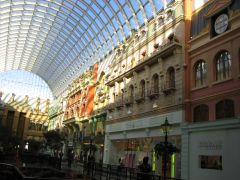
\includegraphics[width=.45\columnwidth]{Lorem}} \quad
\subfloat[Pan ma signo]
{\label{fig:example-b}%
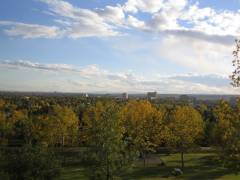
\includegraphics[width=.45\columnwidth]{Ipsum}} \\
\subfloat[Methodicamente o uno]
{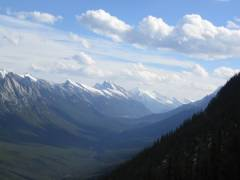
\includegraphics[width=.45\columnwidth]{Dolor}} \quad
\subfloat[Titulo debitas]
{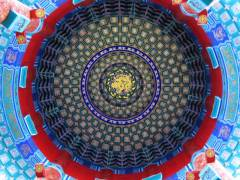
\includegraphics[width=.45\columnwidth]{Sit}}
\caption[Tu duo titulo debitas latente]{Tu duo titulo debitas latente}
\label{fig:example}
\end{figure}

Please note that the content of this section is just some dummy text. It isn't a real language.

Lorem ipsum dolor sit amet, consectetuer adipiscing elit. Ut purus elit, vestibulum ut, placerat ac, adipiscing vitae, felis. Curabitur dictum gravida mauris.

\subsection*{A subsection}

\lipsum[2]

\subsubsection*{A sub-subsection}

\lipsum[7]

\paragraph{A paragraph}
Lorem ipsum dolor sit amet, consectetuer adipiscing elit. Ut purus elit, vestibulum ut, placerat ac, adipiscing vitae, felis. Curabitur dictum gravida mauris. Nam arcu libero, nonummy eget, consectetuer id, vulputate a, magna.

\paragraph{Another paragraph}
Cras nec ante, pellentesque a nulla, cum sociis natoque penatibus et magnis dis parturient montes, nascetur ridiculus mus. Aliquam tincidunt urna

\bigskip

Donec aliquet, tortor sed accumsan bibendum, erat ligula aliquet magna, vitae ornare odio metus a mi. Morbi ac orci et nisl hendrerit mollis. Suspendisse ut massa. Cras nec ante. Pellentesque a nulla. Cum sociis natoque penatibus et magnis dis parturient montes, nascetur ridiculus mus. Aliquam tincidunt urna.

\begin{description}
\item[Mane] Lorem ipsum dolor sit amet, consectetuer adipiscing elit.
\item[Tekel] Ut purus elit, vestibulum ut, placerat ac, adipiscing vitae, felis. Curabitur dictum gravida mauris.
\item[Fares] Nam arcu libero, nonummy eget, consectetuer
id, vulputate a, magna.
\end{description}

\begin{table}
\caption{Lorem ipsum dolor sit amet}
\centering
\begin{tabular}{ll}
\toprule
\textbf{Alkaloid} & \textbf{Origin} \\
\midrule
atropine & belladonna \\
morphine & poppy \\
nicotine & tobacco \\
\bottomrule
\end{tabular}
\end{table}

Suspendisse vel felis. Ut lorem lorem, interdum eu, tincidunt sit amet, laoreet vitae, arcu. Aenean faucibus pede eu ante. Praesent enim elit, rutrum at, molestie non, nonummy vel, nisl. Ut lectus eros, malesuada sit amet, fermentum eu, sodales cursus, magna. Donec eu purus. Quisque vehicula, urna sed ultricies auctor, pede lorem egestas dui, et convallis elit erat sed nulla.

\subsection*{Some formulas}

Una formula in linea viene incorporata nel testo: $\lim_{n \to \infty}\sum_{k=1}^n \frac{1}{k^2} = \frac{\pi^2}{6}$, per esempio. Come si osserva, \LaTeX{} fa \emph{il possibile} per comprimerla e modificare il meno possibile l'interlinea nel capoverso che la contiene.
Una formula in display viene invece composta da \LaTeX{} su linee a parte, separate dal contesto con adeguati spazi bianchi per metterla in mostra e farla risaltare sulla pagina.
\begin{equation}
\lim_{n \to \infty}\sum_{k=1}^n \frac{1}{k^2}= \frac{\pi^2}{6}
\end{equation}
Come si osserva, ora la formula risulta centrata, non compressa, e tutti i suoi elementi occupano il giusto spazio con un risultato finale di grande respiro.

Integer tempus convallis augue. Etiam facilisis. Nunc elementum fermentum wisi. Aenean placerat. Ut imperdiet, enim sed gravida sollicitudin, felis odio placerat quam, ac pulvinar elit purus eget enim.

\begin{equation}
\int_a^{a+T}f(x)\,dx= \int_0^T f(x)\,dx
\qquad
\oint f(z)\,dz=2\pi i
\end{equation}

Nulla malesuada porttitor diam. Donec felis erat, congue non, volutpat at, tincidunt tristique, libero. Vivamus viverra fermentum felis. Donec non- ummy pellentesque ante.

\begin{equation}
f(x_1,\dots,x_n)=  \prod_{k=1}^n x_k
\qquad
\sum_{k=1}^n x_k^2=1
\qquad
\biggl(\sum_n x_n^2\biggr)^{1/2}
\end{equation}

\lipsum[2]

\begin{equation}
\begin{bmatrix}
a_{11} & \dots & a_{1n} \\
a_{21} & \dots & a_{2n} \\
\hdotsfor{3} \\
a_{n1} & \dots & a_{nn}
\end{bmatrix}
\end{equation}

\lipsum[4]

\begin{equation}
\lim_{x\to 0}
\frac{\sin x}{x}=1 \qquad
\lim_{n\to +\infty}f_n=\delta
\end{equation}

Fusce mauris. Vestibulum luctus nibh at lectus. Sed bibendum, nulla a faucibus semper, leo velit ultricies tellus, ac venenatis arcu wisi vel nisl. Vestibulum diam.

\begin{equation}
n!=
\begin{cases}
1       & \text{if $n=0$} \\
n(n-1)! & \text{if $n\ge 1$}
\end{cases}
\end{equation}

Ut lectus eros, malesuada sit amet, fermentum eu, sodales cursus, magna. Donec eu purus. Quisque vehicula, urna sed ultricies auctor, pede lorem egestas dui, et convallis elit erat sed nulla. Donec luctus. Curabitur et nunc. Aliquam dolor odio, commodo pretium, ultricies non, pharetra in, velit.

\begin{equation}
x_G=
\frac{\displaystyle
      \sum_{i=1}^n m_ix_i}
{\displaystyle\sum_{i=1}^n m_i}
\end{equation}

\lipsum[6]

\begin{equation}
\kappa =\frac{\xi}{E_{\textrm{max}}}
\qquad
E_{\textup{max}} =\frac{2 m_{\textup{e}} \beta^2\gamma^2 }{1 +2\gamma m_{\textup{e}}/m_{\textrm{x}} + ( m_{\textup{e}}/m_{\textup{x}})^2}
\end{equation}

\lipsum[8]

%% !TEX TS-program = pdflatex
% !TEX root = ../tesi.tex

%************************************************
\chapter{Code}
\label{chp:code}
%************************************************

\lstset{numbers=left,
    numberstyle=\scriptsize,
    stepnumber=1,
    numbersep=8pt
}



Package announcement and request for necessary packages.
\begin{lstlisting}[firstnumber=1]
\NeedsTeXFormat{LaTeX2e}
\ProvidesPackage{arsclassica}[2017/02/01]
\RequirePackage{classicthesis}
\RequirePackage{caption}
\end{lstlisting}



Text body size.
\begin{lstlisting}
\areaset[current]{370pt}{784pt}
\end{lstlisting}



Use of Iwona as font sans serif.
\begin{lstlisting}
\renewcommand{\sfdefault}{iwona}
\end{lstlisting}



Customized chapter numbers.
\begin{lstlisting}
\let\chapterNumber\undefined
\ifct@eulerchapternumbers
\newfont{\chapterNumber}{eurb10 scaled 5000}%
\else
\newfont{\chapterNumber}{pplr9d scaled 5000}%
\fi
\end{lstlisting}



Smallcaps sans serif.
\begin{lstlisting}
\ifthenelse{\boolean{@minionprospacing}}%
{%
  \DeclareRobustCommand{\spacedallcaps}[1]{\sffamily%
  \textssc{\MakeTextUppercase{#1}}}%
  \DeclareRobustCommand{\spacedlowsmallcaps}[1]%
  {\sffamily\textssc{\MakeTextLowercase{#1}}}%
}{%
  \ifthenelse{\boolean{@pdfspacing}}%
  {%
    \microtypesetup{expansion=false}%
    \DeclareRobustCommand{\spacedallcaps}[1]%
    {\sffamily\textls[160]{\MakeTextUppercase{#1}}}%
    \DeclareRobustCommand{\spacedlowsmallcaps}[1]%
    {\sffamily\textls[80]{\scshape\MakeTextLowercase{#1}}}%
  }{%
    \RequirePackage{soul}
    \sodef\allcapsspacing{\sffamily\upshape}%
    {0.15em}{0.65em}{0.6em}%
    \sodef\lowsmallcapsspacing{\sffamily\scshape}%
    {0.075em}{0.5em}{0.6em}%
    \DeclareRobustCommand{\spacedallcaps}[1]%
    {\MakeTextUppercase{\allcapsspacing{#1}}}%
	\DeclareRobustCommand{\spacedlowsmallcaps}[1]%
	{\MakeTextLowercase{\textsc%
	   {\lowsmallcapsspacing{#1}}}}%
  }%
}
\end{lstlisting}



Semi-transparent headlines and page numbers in Iwona.
\begin{lstlisting}
\renewcommand{\sectionmark}[1]{\markright{\textsc%
{\MakeTextLowercase{\thesection}} \spacedlowsmallcaps{#1}}}
\lehead{\mbox{\llap{\small\thepage\kern1em\color{halfgray}\vline}%
\color{halfgray}\hspace{0.5em}\headmark\hfil}}
\rohead{\mbox{\hfil{\color{halfgray}%
\headmark\hspace{0.5em}}%
\rlap{\small{\color{halfgray}\vline}\kern1em\thepage}}}
\renewcommand{\headfont}{\normalfont\sffamily}
\renewcommand{\pnumfont}{\small\sffamily}
\end{lstlisting}



Sectioning unit titles and description list labels in Iwona.
\begin{lstlisting}
\RequirePackage{titlesec}
    % parts
    \ifthenelse{\boolean{@parts}}%
    {%
    \titleformat{\part}[display]
        {\normalfont\centering\large}%
        {\thispagestyle{empty}\partname~\thepart}{1em}%
        {\color{Maroon}\spacedallcaps}
    }{\relax}
    % chapters
    \ifthenelse{\boolean{@linedheaders}}%
    {%
    \titleformat{\chapter}[display]%
       {\relax}{\raggedleft{\color{halfgray}%
       \chapterNumber\thechapter} \\ }{0pt}%
       {\titlerule\vspace*{.9\baselineskip}\raggedright%
       \spacedallcaps}%
       [\normalsize\vspace*{.8\baselineskip}\titlerule]%
    }{%
    \titleformat{\chapter}[block]%
       {\normalfont\Large\sffamily}%
       {{\color{halfgray}\chapterNumber\thechapter%
       \hspace{10pt}\vline}  }{10pt}%
       {\spacedallcaps}}
    % sections
    \titleformat{\section}
       {\normalfont\Large\sffamily}{\textsc%
       {\MakeTextLowercase{\thesection}}}%
       {1em}{\spacedlowsmallcaps}
    % subsections
       \titleformat{\subsection}
       {\normalfont\sffamily\bfseries}{\textsc{\MakeTextLowercase%
       {\thesubsection}}}{1em}{\normalsize}
    % subsubsections
    \titleformat{\subsubsection}
       {\normalfont\sffamily\bfseries\itshape}{\textsc%
       {\MakeTextLowercase{\thesubsubsection}}}%
       {1em}{\normalsize\itshape}
    % paragraphs
    \titleformat{\paragraph}[runin]
       {\normalfont\normalsize\sffamily\bfseries}{\textsc%
       {\MakeTextLowercase{\theparagraph}}}%
       {0pt}{\spacedlowsmallcaps}
    % description labels
    \renewcommand{\descriptionlabel}[1]{\hspace*{\labelsep}%
    \bfseries\spacedlowsmallcaps{#1}}
    \titlespacing*{\chapter}{0pt}{1\baselineskip}{2\baselineskip}
    \titlespacing*{\section}{0pt}{2\baselineskip}%
       {.8\baselineskip}[\marginparsep]
    \titlespacing*{\subsection}{0pt}{1.5\baselineskip}%
       {.8\baselineskip}[\marginparsep]
    \titlespacing*{\paragraph}{0pt}{1\baselineskip}{1\baselineskip}

    \newcommand\formatchapter[1]{%
    \vbox to \ht\strutbox{
    \setbox0=\hbox{\chapterNumber\thechapter\hspace{10pt}\vline\ }
    \advance\hsize-\wd0 \advance\hsize-10pt\raggedright
    \spacedallcaps{#1}\vss}}
    \titleformat{\chapter}[block]
       {\normalfont\Large\sffamily}
       {\textcolor{halfgray}{\chapterNumber\thechapter}
       \hspace{10pt}\vline\ }{10pt}
    {\formatchapter}

    \clearscrplain
    \rofoot[\mbox{\makebox[0pt][l]{\kern1em\thepage}}]{}
\end{lstlisting}



Itemize lists with semi-transparent labels.
\begin{lstlisting}
\renewcommand\labelitemi{\color{halfgray}$\bullet$}
\end{lstlisting}



Caption settings.
\begin{lstlisting}
\captionsetup{format=hang,font=small,labelfont={sf,bf}}
\captionsetup[table]{skip=\medskipamount}
\end{lstlisting}



Hyper-reference settings.
\begin{lstlisting}
\hypersetup{
    colorlinks=true, linktocpage=true, pdfstartpage=1,
    pdfstartview=FitV, breaklinks=true, pdfpagemode=UseNone,
    pageanchor=true, pdfpagemode=UseOutlines,
    plainpages=false, bookmarksnumbered,
    bookmarksopen=true, bookmarksopenlevel=1,
    hypertexnames=true, pdfhighlight=/O,
    urlcolor=webbrown, linkcolor=RoyalBlue,
    citecolor=webgreen,
    hyperfootnotes=false, pdfpagelabels,
    pdfcreator={pdfLaTeX},
    pdfproducer={LaTeX with ArsClassica}
}
\end{lstlisting}

\clearpage
% !TEX TS-program = pdflatex
% !TEX root = ../tesi.tex

%*******************************************************
% Bibliography
%*******************************************************
\nocite{*}
\printbibliography

\end{document}
